%%%%%%%%%%%%%%%%%%%%%%%%%%%%%%%%%%%%%%%%%%%%%%%%%%%%%%%%%%
%%%%%%%%%%%%%%%%%%%%%%%%%%%%%%%%%%%%%%%%%%%%%%%%%%%%%%%%%%
%
%                                        PRE-AMBLE
%
%%%%%%%%%%%%%%%%%%%%%%%%%%%%%%%%%%%%%%%%%%%%%%%%%%%%%%%%%%
%%%%%%%%%%%%%%%%%%%%%%%%%%%%%%%%%%%%%%%%%%%%%%%%%%%%%%%%%%

\documentclass[11pt]{amsart}

\setlength{\textwidth}{\paperwidth}
\addtolength{\textwidth}{-3in}
\calclayout

%LOAD PACKAGES--------------------------------------------

\usepackage{amsfonts, amsthm, amssymb, amsmath, stmaryrd, etoolbox}
\usepackage{comment}
\usepackage{mathtools}
\usepackage{graphicx,caption,subcaption}
\usepackage{todonotes}
\usepackage{xcolor}

\usepackage[inline]{enumitem}
\setlist{itemsep=0em, topsep=0em, parsep=0em}
\setlist[enumerate]{label=(\alph*)}

\usepackage{tikz}
\usepackage[all,2cell]{xy}
\usetikzlibrary{matrix,arrows,shapes,decorations.markings,decorations.pathreplacing}
\definecolor{rewritecolor}{rgb}{0,.9,1}
\tikzset{rewritenode/.style={shape=circle,fill=rewritecolor,scale=0.25,font=\Huge}}
\tikzset{RWopen/.style={shape=circle,draw=black,fill=white,scale=0.5,font=\Huge}}
\tikzset{RWclosed/.style={shape=circle,fill=black,scale=0.5,font=\Huge}}
\tikzset{CDnode/.style={shape=circle,fill=white,scale=.5}}
\tikzset{zxgreen/.style={shape=circle,draw,fill=green}}
\tikzset{zxred/.style={shape=circle,draw,fill=red}}
\tikzset{zxyellow/.style={shape=rectangle,draw,fill=yellow,inner sep=2.75}}
\tikzset{zxdiamond/.style={shape=diamond,fill=black,inner sep=2.75}}
\tikzset{zxopen/.style={shape=circle,draw,inner sep=2pt}}
\tikzset{->-/.style={decoration={markings,mark=at position .5 with {\arrow{>}}},postaction={decorate}}}

\usepackage{hyperref}
\definecolor{hyperrefcolor}{rgb}{0,0,0.7}
\hypersetup{colorlinks,linkcolor={hyperrefcolor},citecolor={hyperrefcolor},urlcolor={hyperrefcolor}}

%NEW COMMANDS---------------------------------------------

\newcommand{\RR}{\mathbb{R}}
\newcommand{\ZZ}{\mathbb{Z}}
\newcommand{\NN}{\mathbb{N}}
\newcommand{\QQ}{\mathbb{Q}}
\newcommand{\CC}{\mathbb{C}}
\renewcommand{\epsilon}{\varepsilon}

\newcommand{\cl}[1]{\mathcal{#1}}
\newcommand{\scr}[1]{\mathscr{#1}}
\newcommand{\op}[1]{\operatorname{#1}}
\newcommand{\cat}[1]{\mathbf{#1}}
\newcommand{\dblcat}[1]{\mathbb{#1}}
\renewcommand{\t}[1]{\textup{#1}}

\newcommand{\from}{\colon}
\newcommand{\xto}[1]{\xrightarrow{#1}}
\newcommand{\sm}{\smallsetminus}
\newcommand{\tospan}{\xrightarrow{\mathit{sp}}}
\newcommand{\tocospan}{\xrightarrow{\mathit{csp}}}

%\newcommand{\diagram}[1]{\raisebox{-0.5\height}{\includegraphics{#1}}}

\newcommand{\bluebullet}{\textcolor{rewritecolor}{\bullet}}

%  macros for (co)span bicategories
\newcommand{\bispmap}[1]{\mathbf{Sp(#1)}}
\newcommand{\dblspmap}[1]{\mathbb{S}\mathbf{p(#1)}}
\newcommand{\bicspmap}[1]{\mathbf{Csp(#1)}}
\newcommand{\dblcspmap}[1]{\mathbb{C}\mathbf{sp(#1)}}
\newcommand{\bispsp}[1]{\mathbf{Sp(Sp(#1))}}
\newcommand{\dblspsp}[1]{\mathbb{S}\mathbf{p(Sp(#1))}}
\newcommand{\bicspcsp}[1]{\mathbf{Csp(Csp(#1))}}
\newcommand{\dblcspcsp}[1]{\mathbb{C}\mathbf{sp(Csp(#1))}}
\newcommand{\bimonspcsp}[1]{\mathbf{MonicSp(Csp(#1))}}
\newcommand{\dblmonspcsp}[1]{\mathbb{M}\mathbf{onicSp(Csp(#1))}}
\newcommand{\biepiccspsp}[1]{\mathbf{EpicCsp(Sp(#1))}}
\newcommand{\dblepiccspsp}[1]{\mathbb{E}\mathbf{picCsp(Sp(#1))}}

% defining arrow with a vertical line through it
\makeatletter
\def\slashedarrowfill@#1#2#3#4#5{%
	$\m@th\thickmuskip0mu\medmuskip\thickmuskip\thinmuskip\thickmuskip
	\relax#5#1\mkern-7mu%
	\cleaders\hbox{$#5\mkern-2mu#2\mkern-2mu$}\hfill
	\mathclap{#3}\mathclap{#2}%
	\cleaders\hbox{$#5\mkern-2mu#2\mkern-2mu$}\hfill
	\mkern-7mu#4$%
}
\def\rightslashedarrowfill@{%
	\slashedarrowfill@\relbar\relbar\mapstochar\rightarrow}
\newcommand{\xslashedrightarrow}[2][]{%
	\ext@arrow 0055{\rightslashedarrowfill@}{#1}{#2}}
\makeatother

\newcommand{\hto}{\xslashedrightarrow{}}


%DECLARE MATH OPERATORS----------------------------------

\DeclareMathOperator{\Hom}{Hom}
\DeclareMathOperator{\id}{id}
\DeclareMathOperator{\ob}{Ob}
\DeclareMathOperator{\arr}{arr}
\DeclareMathOperator{\im}{im}
\DeclareMathOperator{\Aut}{Aut}
\DeclareMathOperator{\Bij}{Bij}
\DeclareMathOperator{\Sub}{Sub}

%ENVIRONMENTS AND COUNTERS---------------------------------

\newtheorem{thm}{Theorem}[section]
\newtheorem{lem}[thm]{Lemma}
\newtheorem{prop}[thm]{Proposition}
\newtheorem{cor}[thm]{Corollary}

\theoremstyle{remark}
\newtheorem{remark}[thm]{Remark}
\newtheorem{notation}[thm]{Notation}

\theoremstyle{definition}
\newtheorem{ex}[thm]{Example} 
\newtheorem{defn}[thm]{Definition}

%\setcounter{tocdepth}{1} % Sets depth for table of contents. 

%%%%%%%%%%%%%%%%%%%%%%%%%%%%%%%%%%%%%%%%%%%%%%%%%%%%%%%%%
%%%%%%%%%%%%%%%%%%%%%%%%%%%%%%%%%%%%%%%%%%%%%%%%%%%%%%%%%
%%%%%%%%%%%%%%%%%%%%%%%%%%%%%%%%%%%%%%%%%%%%%%%%%%%%%%%%%
%%%%%%%%%%%%%%%%%%%%%%%%%%%%%%%%%%%%%%%%%%%%%%%%%%%%%%%%%
%
%BEGIN DOCUMENT
%
%%%%%%%%%%%%%%%%%%%%%%%%%%%%%%%%%%%%%%%%%%%%%%%%%%%%%%%%%
%%%%%%%%%%%%%%%%%%%%%%%%%%%%%%%%%%%%%%%%%%%%%%%%%%%%%%%%%
%%%%%%%%%%%%%%%%%%%%%%%%%%%%%%%%%%%%%%%%%%%%%%%%%%%%%%%%%
%%%%%%%%%%%%%%%%%%%%%%%%%%%%%%%%%%%%%%%%%%%%%%%%%%%%%%%%%

\begin{document}
	
%\tableofcontents

\begin{abstract}
	It was shown in \cite{Cic} that given a topos $T$, we can form a bicategory $\bimonspcsp{T}$ whose $0$-cells are the $T$-objects, $1$-cells are cospans in $T$, and $2$-cells are spans of cospans with monic legs. Taking $T$ to be the category $\cat{Graph}$ of (directed) graphs and graph morphisms, we consider the full sub-bicategory $\cat{Rewrite}$ of $\bimonspcsp{Graph}$ on the edgeless graphs. This bicategory ought to be considered as having open graphs and ways of rewriting them.  We then demonstrate that we can capture categories of graphs with extra structure by considering certain slice categories of $\cat{Graph}$.  We can then construct a symmetric monoidal, compact closed bicategory of open structured graphs and their rewritings.  Finally, we apply this construction to categorify the PROP whose morphisms are diagrams in the zx-calculus developed by Coecke and Duncan.
\end{abstract}

\title{Rewriting on open structured graphs}
\author{Daniel Cicala}
\maketitle

%%%%%%%%%%%%%%%%%%%%%%%%%%%%%%%%%%%%%%%%%%%%%%%%%%%%%%%%%
%%%%%%%%%%%%%%%%%%%%%%%%%%%%%%%%%%%%%%%%%%%%%%%%%%%%%%%%%
% INTRODUCTION
\section{Introduction}
\label{sec:Intro}
%%%%%%%%%%%%%%%%%%%%%%%%%%%%%%%%%%%%%%%%%%%%%%%%%%%%%%%%%
%%%%%%%%%%%%%%%%%%%%%%%%%%%%%%%%%%%%%%%%%%%%%%%%%%%%%%%%%

%%%%%%%%%%%%%%%%%%%%%%%%%%%%%%%%%%%%%%%%%%%%%%%%%%%%%%%%%
%%%%%%%%%%%%%%%%%%%%%%%%%%%%%%%%%%%%%%%%%%%%%%%%%%%%%%%%%
% A BICATEGY FOR REWRITING OPEN GRAPHS
\section{Rewriting open graphs}
\label{subsec:RewritingOpenGraphs}
%%%%%%%%%%%%%%%%%%%%%%%%%%%%%%%%%%%%%%%%%%%%%%%%%%%%%%%%%
%%%%%%%%%%%%%%%%%%%%%%%%%%%%%%%%%%%%%%%%%%%%%%%%%%%%%%%%%

Intuitively, the notion of an open graph is rather simple.  Take a directed graph and declare some of the nodes to be inputs and others to be outputs, for instance
\[
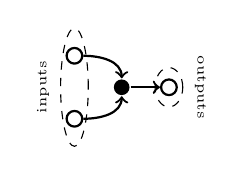
\begin{tikzpicture}
	\begin{scope}
	\node [circle,draw,inner sep=2pt,thick] (1) at (-.2,0) {};
	\node [circle,fill,inner sep=2pt,thick] (2) at (-.8,0) {};
	\node [circle,draw,inner sep=2pt,thick] (3) at (-1.4,0.4) {};
	\node [circle,draw,inner sep=2pt,thick] (4) at (-1.4,-0.4) {};
	%
	\draw [thick,->] (4) edge[out=0,in=-90] (2);
	\draw [thick,->] (3) edge[out=0,in=90] (2);
	\draw [thick,->] (2) edge (1);
	%
	\draw [dashed] (-1.4,0) ellipse (0.5em and 0.75cm);
	\node [rotate=90] at (-1.8,0) {\tiny inputs};
	\draw [dashed] (-0.2,0) ellipse (0.5em and 0.25cm);
	\node [rotate=-90] at (0.2,0) {\tiny outputs};
	\end{scope}
\end{tikzpicture}
\]
Whenever there is a bijection between the inputs of one graph and the outputs of another, we can connect them in a way described by the bijection.  This process is provides a way to turn a pair of compatible open graphs into a single open graph.  Indeedn, we cannot connect 
\[
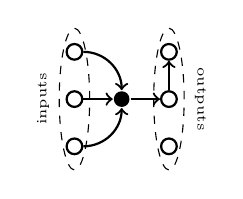
\begin{tikzpicture}
	\begin{scope}
	\node [circle,draw,inner sep=2pt,thick] (1) at (-.2,0.6) {};
	\node [circle,draw,inner sep=2pt,thick] (2) at (-.2,0) {};
	\node [circle,draw,inner sep=2pt,thick] (3) at (-.2,-0.6) {};
	\node [circle,fill,inner sep=2pt,thick] (4) at (-.8,0) {};
	\node [circle,draw,inner sep=2pt,thick] (5) at (-1.4,0.6) {};
	\node [circle,draw,inner sep=2pt,thick] (6) at (-1.4,0) {};
	\node [circle,draw,inner sep=2pt,thick] (7) at (-1.4,-0.6) {};
	%
	\draw [thick,->] (7) edge[out=0,in=-90] (4);
	\draw [thick,->] (6) edge (4);
	\draw [thick,->] (5) edge[out=0,in=90] (4);
	\draw [thick,->] (4) edge (2);
	\draw [thick,->] (2) edge (1);
	%
	\draw [dashed] (-1.4,0) ellipse (0.55em and 0.9cm);
	\node [rotate=90] at (-1.8,0) {\tiny inputs};
	\draw [dashed] (-0.2,0) ellipse (0.55em and 0.9cm);
	\node [rotate=-90] at (0.2,0) {\tiny outputs};
	\end{scope}
\end{tikzpicture}
\]
to the above open graph, though we can connect 
\[
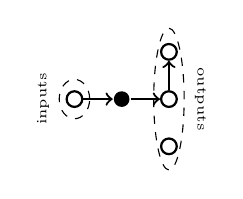
\begin{tikzpicture}
	\begin{scope}
	\node [circle,draw,inner sep=2pt,thick] (1) at (-.2,0.6) {};
	\node [circle,draw,inner sep=2pt,thick] (2) at (-.2,0) {};
	\node [circle,draw,inner sep=2pt,thick] (3) at (-.2,-0.6) {};
	\node [circle,fill,inner sep=2pt,thick] (4) at (-.8,0) {};
	\node [circle,draw,inner sep=2pt,thick] (6) at (-1.4,0) {};
	%
	\draw [thick,->] (6) edge (4);
	\draw [thick,->] (4) edge (2);
	\draw [thick,->] (2) edge (1);
	%
	\draw [dashed] (-1.4,0) ellipse (0.55em and 0.25cm);
	\node [rotate=90] at (-1.8,0) {\tiny inputs};
	\draw [dashed] (-0.2,0) ellipse (0.55em and 0.9cm);
	\node [rotate=-90] at (0.2,0) {\tiny outputs};
	\end{scope}
\end{tikzpicture}
\]
to form the open graph
\[
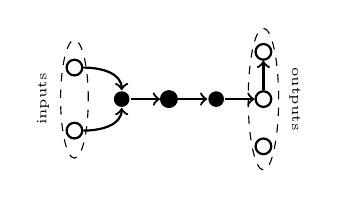
\begin{tikzpicture}
	\begin{scope}[shift={(0.2,0)}]
	\node [circle,fill,inner sep=2pt,thick] (1) at (-.2,0) {};
	\node [circle,fill,inner sep=2pt,thick] (2) at (-.8,0) {};
	\node [circle,draw,inner sep=2pt,thick] (3) at (-1.4,0.4) {};
	\node [circle,draw,inner sep=2pt,thick] (4) at (-1.4,-0.4) {};
	%
	\draw [thick,->] (4) edge[out=0,in=-90] (2);
	\draw [thick,->] (3) edge[out=0,in=90] (2);
	\draw [thick,->] (2) edge (1);
	%
	\draw [dashed] (-1.4,0) ellipse (0.5em and 0.75cm);
	\node [rotate=90] at (-1.8,0) {\tiny inputs};
	\end{scope}
	%
	%
	%
	\begin{scope}[shift={(1.4,0)}]
	\node [circle,draw,inner sep=2pt,thick] (1) at (-.2,0.6) {};
	\node [circle,draw,inner sep=2pt,thick] (2) at (-.2,0) {};
	\node [circle,draw,inner sep=2pt,thick] (3) at (-.2,-0.6) {};
	\node [circle,fill,inner sep=2pt,thick] (4) at (-.8,0) {};
	\node [circle,draw,inner sep=2pt,thick] (6) at (-1.4,0) {};
	%
	\draw [thick,->] (6) edge (4);
	\draw [thick,->] (4) edge (2);
	\draw [thick,->] (2) edge (1);
	%
	\draw [dashed] (-0.2,0) ellipse (0.55em and 0.9cm);
	\node [rotate=-90] at (0.2,0) {\tiny outputs};
	\end{scope}
\end{tikzpicture}
\]

This is made precise using cospans and pushout as follows. Consider the functor $N \from \cat{Set} \to \cat{Graph}$ that assigns the edgeless graph with node set $X$ to a set $X$.  An \emph{open graph} is then a cospan in the category $\cat{Graph}$ of the form $N(X) \to G \gets N(Y)$ for sets $X$ and $Y$. We will denote this open graph by $G$ when the legs of the cospan do not need to be explicit.  Also, call the left leg $N(X)$ of the cospan the \emph{inputs} of $G$ and the right leg $N(Y)$ the \emph{outputs} of $G$.  Suppose we have another open graph $G'$ with inputs $N(Y)$ and outputs $N(Z)$.  Then we can compose the cospans 
\[
	N(X) \to G \gets N(Y) \to G' \gets N(Z). 
\] 
This is certainly not an open graph, but pushing out over the span $G \gets N(Y) \to G'$ induces the open graph  
\[
	N(X) \to G +_{N(Y)} G' \gets N(Z).
\] 
By taking isomorphism classes of these pushouts, we obtain a category whose objects are those in the image of $N$ and morphisms are open graphs. 

But we can do better! Indeed, we have only just described the first layer of a symmetric monoidal and compact closed bicategory. This bicategory was introduced by the author in \cite{Cic} under the name $\cat{Rewrite}$. It was shown that $\cat{Rewrite}$ is symmetric monoidal and compact closed in a joint work with Courser \todo{cite here}. Before moving on to consider graphs equipped with some additional structure, we briefly recall the story of $\cat{Rewrite}$.

Given a topos $\cat{T}$, there is a symmetric monoidal and compact closed bicategory $\bimonspcsp{T}$ consisting of 
\begin{itemize}
	\item (0-cells) objects of $\cat{T}$,
	\item (1-cells) cospans in $\cat{T}$, and
	\item (2-cells) isoclasses of monic spans of cospans in $\cat{T}$.
\end{itemize} 
The 2-cells are diagrams 
\[
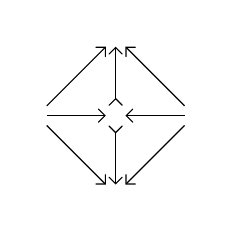
\begin{tikzpicture}
	\node (A) at (0,0) {};
	\node (B) at (1,1) {};
	\node (B') at (1,0) {};
	\node (B'') at (1,-1) {};
	\node (C) at (2,0) {};
	%
	\path[->,font=\scriptsize,>=angle 90]
	(A) edge node[above]{$$} (B)
	(A) edge node[above]{$$} (B')
	(A) edge node[above]{$$} (B'')
	(C) edge node[above]{$$} (B)
	(C) edge node[above]{$$} (B')
	(C) edge node[left]{$$} (B'')
	(B') edge[>->] node[right]{$$} (B)
	(B') edge[>->] node[left]{$$} (B'');
\end{tikzpicture}
\] 
where `$\rightarrowtail$' denotes a monic $\cat{T}$-morphism.  Because $\bimonspcsp{T}$ is such a long name, we will shorten it to $\cat{MSC}(\cat{T})$.

Letting $\cat{T}$ be the topos $\cat{Graph}$ of directed graphs, there is a symmetric monoidal and compact closed sub-bicategory of $\bimonspcsp{Graph}$ called $\cat{Rewrite}$ whose $0$-cells are exactly the edgeless graphs, and full in $1$-cells and $2$-cells. The idea of $\cat{Rewrite}$ is that the $1$-cells are open graphs and the $2$-cells are the ways to rewrite a graph into another while preserving the input and output nodes. By rewriting, we mean double pushout graph rewriting \todo{DPO citation}. This means that restricting ourselves to monic spans in the $2$-cells is not overly restrictive since many authors only consider monic double pushout rewriting rules.  

The motivation for constructing $\cat{Rewrite}$ is not necessarily to study it directly, but rather for it to serve as an ambient context in which to generate symmetric monoidal and compact closed sub-bicategories on some collection of open graphs and rewriting rules. Of course, the collection that one would use depends on their interest. To illustrate, Example \todo{put frob algebra example here} in \todo{cite Kenny/me} shows that we obtain a categorified version of $\cat{2Cob}$, the category of \todo{describe 2cob here}, with the following generators: \todo{input generators}

Why care about $\cat{Rewrite}$? Graphical calculi typically use some version of open graphs as a semantics and equations between graphical terms are given by rewrite rules \todo{citeation here}. However, equations are evil when looking through a categorical lens.  Morally, equations ought to be replaced by isomorphisms. The process of replacing equations with isomorphisms and sets by categories is known as categorification. In this program, we are interested in categorifying certain categories into bicategories. The categories of interest are those whose morphisms are associated to open graphs of some sort. For instance there are a number of categories of open networks \todo{cite papers here} which we seek to categorify by interpreting rewrite rules as $2$-cells instead of as providing equations between morphisms.  However, this requires some work.

There are drawbacks to this approach. For example, working with open graphs is only useful to model graphical calculi whose terms are equal up to isotopy in $4$ dimensions \todo{expand on this}. Amending $\cat{Rewrite}$ to account for this shortcoming is a direction of future research.  Currently, our interest lies in expanding the idea of $\cat{Rewrite}$ to account for `open structured graphs', which we introduce in the next section.  

%%%%%%%%%%%%%%%%%%%%%%%%%%%%%%%%%%%%%%%%%%%%%%%%%%%%%%%%%
%%%%%%%%%%%%%%%%%%%%%%%%%%%%%%%%%%%%%%%%%%%%%%%%%%%%%%%%%
% OPEN STRUCTURED GRAPHS
\section{Open structured graphs}
\label{subsec:OpenStructuredGraphs}
%%%%%%%%%%%%%%%%%%%%%%%%%%%%%%%%%%%%%%%%%%%%%%%%%%%%%%%%%
%%%%%%%%%%%%%%%%%%%%%%%%%%%%%%%%%%%%%%%%%%%%%%%%%%%%%%%%%

So far, we have seen that there is a symmetric monoidal and compact closed bicategory $\cat{MSC}(\cat{T})$ for any topos $\cat{T}$. Moreover, when $\cat{T} \coloneqq \cat{Graph}$, we get this nice symmetric monoidal and compact closed sub-bicategory $\cat{Rewrite}$. Because many graphical languages use graphs with additional structure, it would be nice to give a similar construction for these cases. To this end, we first discuss a method of providing additional structure in a manner that is amenable to this construction.

Let $S$ be a graph.  By a graph over $S$, we mean a graph morphism $G \to S$. Then a morphism between graphs over $S$ is a graph morphism $G \to G'$ such that 
	\[
	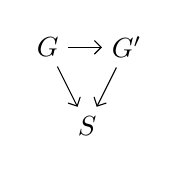
\begin{tikzpicture}
		\node (1) at (-0.5,1) {$G$};
		\node (2) at (0.5,1) {$G'$};
		\node (3) at (0,0) {$S$};
		%
		\path[->,font=\scriptsize,>=angle 90]
		(1) edge (2)
		(1) edge (3)
		(2) edge (3);
	\end{tikzpicture}
	\]
The way to think about how a graph $G$ over $S$ gives structure to $G$ is that $S$ classifies the nodes and edges of $G$ via the fibres of the morphism. This method is being investigated by Baez and Courser in an upcoming paper \todo{cite it}.  However, here is an example to illustrate the concept.

\begin{ex}
	A Petri net (without marking or weighted edges) is a bipartite graph whose partitions are called \emph{species} and \emph{transitions}. Let $S_{\text{PN}}$ be the graph
	\begin{equation}
	\label{diag:PetriNet structure graph}
	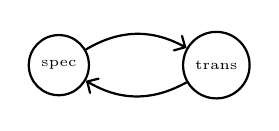
\begin{tikzpicture}[baseline=(current bounding box.center)]
		\node [shape=circle,draw,thick] (T) at (2,0) {\tiny trans};
		\node [shape=circle,draw,thick] (S) at (0,0) {\tiny spec};
		%
		\path[->,thick,font=\scriptsize,>=angle 90]
		(T) edge[bend left] (S)
		(S) edge[bend left] (T);
	\end{tikzpicture}
	\end{equation}
	A Petri net is a graph over $S_{\text{PN}}$. Indeed, given a graph $G$ over $S_{\text{PN}}$, the fibres of the nodes `spec', `trans' are the species and transitions, respectively. The arrows of $S_{\text{PN}}$ force $G$ to be bipartite. For example, the Petri net
	\begin{equation}
	\label{diag:PetriNet example}
	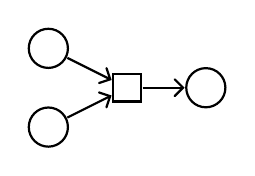
\begin{tikzpicture}[baseline=(current bounding box.center)]
		\node [circle, draw, scale=1.5,thick] (S1) at (0,1) {}; 
		\node [circle, draw, scale=1.5,thick] (S2) at (0,0) {};
		\node [circle, draw, scale=1.5,thick] (S3) at (2,0.5) {};
		\node [rectangle,draw,scale=1.5,thick] (T) at (1,0.5) {};
		%
		\path[->,thick,font=\scriptsize,>=angle 90]
		(S1) edge (T) 
		(S2) edge (T)
		(T) edge (S3);
	\end{tikzpicture}
	\end{equation}
	can be realized as the graph 
	\[
	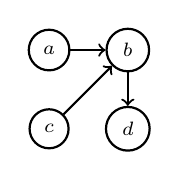
\begin{tikzpicture}
		\node [circle,draw,thick] (a) at (0,1) {\scriptsize $a$};
		\node [circle,draw,thick] (b) at (1,1) {\scriptsize $b$};
		\node [circle,draw,thick] (c) at (0,0) {\scriptsize $c$};
		\node [circle,draw,thick] (d) at (1,0) {\scriptsize $d$};
		%
		\path[->,thick]
		(a) edge (b)
		(c) edge (b)
		(b) edge (d);
	\end{tikzpicture}
	\]
	over $S_{\text{PN}}$ via the assignment $a,c,d \mapsto \text{spec}$ and $b \mapsto \text{trans}$.
\end{ex}

Now, we want to go a bit further and study open graphs over $S$ (for any graph $S$). That is, we want to equip a graph over $S$ with inputs and outputs.  To achieve this, we will use cospans as in the case of $\cat{Rewrite}$ discussed above. Though, the added structure introduces new considerations.

Recall that an over category in a topos is still a topos \todo{find citation}.  In particular, given a graph $S$, we have the topos $\cat{Graph}/S$ of graphs over $S$. It follows that $\cat{MSC}(\cat{Graph}/S)$ is a symmetric monoidal and compact closed bicategory. However, there is not a unique (up to isomorphism) way to be an edgeless graph due to the possibility of there being many graph morphisms to $S$. For instance, the graph $G_2$ with two nodes and no edges can be a graph over $S_{\text{PN}}$ in four different ways because there are four graph morphisms $G_2 \to S_{\text{PN}}$.

However, there is a way to functorially choose edgeless graphs to serve as inputs and outputs for graphs over $S$. Namely, fix a node $\ast$ of $S$ and define a functor $N \from \cat{Set} \to \cat{Graph}/S$ by assigning $N(X) \to S$ to each set $X$ where $N(X)$ is the edgeless graph with nodes $X$ and each node is mapped to $\ast$. 

We will pause here to expand the Petri net example above to an `open Petri net'.  

\begin{ex}
	An open Petri net is a special case of an open graph as defined earlier where only species can be an input or output. However, we want define this using graphs over $S_{\text{PN}}$ from \eqref{diag:PetriNet structure graph}. Define a functor $N \from \cat{Set} \to \cat{Graph}/S_{\text{PN}}$ by sending a set $X$ to $N(X) \to S_{\text{PN}}$ where $N(X)$ is the edgeless graph on the set $X$ and the morphisms is constant over \textit{spec}. An open Petri net is a cospan of the form $N(X) \to P \gets N(Y)$ for sets $X,Y$ and a Petri net $P$ over $S_{\text{PN}}$.  If $P$ is the Petri net from \eqref{diag:PetriNet example}, $X \coloneqq \mathbf{2}$, and $Y \coloneqq \mathbf{1}$, then the picture looks like
	\[
	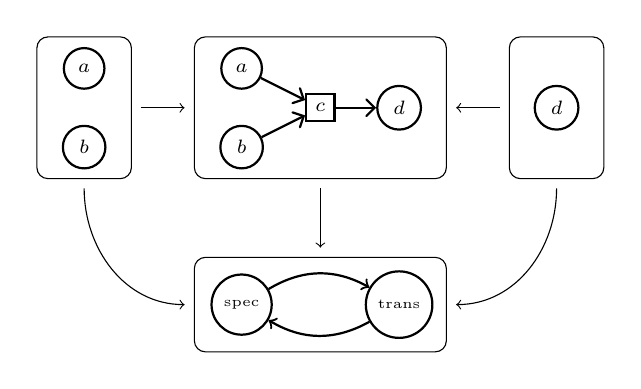
\begin{tikzpicture}
		\begin{scope}[shift={(-3,1)}] %ul graph
		\node [circle, draw,thick] at (0,1) {\scriptsize $a$}; 
		\node [circle, draw,thick] at (0,0) {\scriptsize $b$};
		%
		\node (1) at (-0.6,1.4) {}; %upper left rect corner
		\node (2) at (0.6,-0.4) {}; %lower right rect corner
		\node (ul1) at (0.6,0.5) {}; %anchor for graph map ul-->um
		\node (ul2) at (0,-0.4) {}; %anchor for graph map ul-->l
		\draw [rounded corners] (1) rectangle (2);
		\end{scope}
		%
		%
		%
		\begin{scope}[shift={(-1,1)}] %um graph
		\node [circle, draw,thick] (S1) at (0,1) {\scriptsize $a$}; 
		\node [circle, draw,thick] (S2) at (0,0) {\scriptsize $b$};
		\node [circle, draw,thick] (S3) at (2,0.5) {\scriptsize $d$};
		\node [rectangle,draw,thick] (T) at (1,0.5) {\scriptsize $c$};
		%
		\path[->,thick,font=\scriptsize,>=angle 90]
		(S1) edge (T) 
		(S2) edge (T)
		(T) edge (S3);
		%
		\node (1) at (-0.6,1.4) {}; %upper left rect corner
		\node (2) at (2.6,-0.4) {}; %lower right rect corner
		\node (um1) at (-0.6,0.5) {}; %anchor for graph map ul-->um
		\node (um2) at (1,-0.4) {}; %anchor for graph map um-->l
		\node (um3) at (2.6,0.5) {}; %anchor for graph map ur-->um
		\draw [rounded corners] (1) rectangle (2);
		\end{scope}
		%
		%
		%
		\begin{scope}[shift={(3,1.5)}] %ur graph
		\node [circle, draw,thick] at (0,0) {\scriptsize $d$}; 
		%
		\node (1) at (-0.6,0.9) {}; %upper left rect corner
		\node (2) at (0.6,-0.9) {}; %lower right rect corner
		\node (ur1) at (-0.6,0) {}; %anchor for graph map ur-->um
		\node (ur2) at (0,-0.9) {}; %anchor for graph map ur-->l
		\draw [rounded corners] (1) rectangle (2);
		\end{scope}
		%
		%
		%
		\begin{scope}[shift={(0,-1)}] %l graph
		\node [circle, draw,thick] (S) at (-1,0) {\tiny spec}; 
		\node [circle, draw,thick] (T) at (1,0) {\tiny trans};
		\draw [->,thick] (S) edge[bend left] (T);
		\draw [->,thick] (T) edge[bend left] (S);
		%
		\node (1) at (-1.6,0.6) {}; %upper left rect corner
		\node (2) at (1.6,-0.6) {}; %lower right rect corner
		\node (l1) at (-1.6,0) {}; %anchor for graph map ul-->l
		\node (l2) at (0,0.6) {}; %anchor for graph map um-->l
		\node (l3) at (1.6,0) {}; %anchor for graph map ur-->l
		\draw [rounded corners] (1) rectangle (2);
		\end{scope}
		%
		%
		%
		\begin{scope}
		\draw [->] (ul1) edge[] (um1);
		\draw [->] (ur1) edge[] (um3);
		\draw [->] (ul2) edge[out=-90,in=180] (l1);
		\draw [->] (um2) edge[] (l2);
		\draw [->] (ur2) edge[out=-90,in=0] (l3);
		\end{scope}
	\end{tikzpicture}
	\]
	where the horizontally aligned graph morphisms are defined according to the labeling and the graph morphisms to $S_{\text{PN}}$ send nodes $a,b,d \mapsto \text{spec}$ and $d \mapsto \text{trans}$. Here, we have inputs $a,b$ and output $d$. \todo{go onto composition here?}
\end{ex}

Now that we have a notion of open graphs over $S$, we need to compose compatible such graphs as we did for open graphs.  Again, this is done using pushouts in the category $\cat{Graph}/S$.  

And so in a similar manner to open graphs, given a graph $S$ and a functor $N \from \cat{Set} \to \cat{Graph}/S$ whose object image lies within the collection of edgeless graphs over $S$, we obtain a symmetric monoidal bicategory $\cat{Rewrite}_{N,S}$ contained in $\cat{MSC}(\cat{Graph}/S)$.  The $0$-cells of $\cat{Rewrite}_{N,S}$ are those graphs over $S$ with the form $N(X)$ for a set $X$. Then $\cat{Rewrite}_{N,S}$ is full in the $1$-cells and $2$-cells. Similar to $\cat{Rewrite}$, the usefulness of  $\cat{Rewrite_{N,S}}$ is as an ambient context in which to generate sub-structures on a desired collection of open graphs over $S$ and rewrite rules.  This will be demonstrated on the zx-calculus \todo{cite coerke duncan}. 


%%%%%%%%%%%%%%%%%%%%%%%%%%%%%%%%%%%%%%%%%%%%%%%%%%%%%%%%%
%%%%%%%%%%%%%%%%%%%%%%%%%%%%%%%%%%%%%%%%%%%%%%%%%%%%%%%%%
% THE ZX-CALCULUS AS OPEN STRUCTURED GRAPHS
\section{The zx-calculus as open structured graphs}
\label{sec:ZxCalc}
%%%%%%%%%%%%%%%%%%%%%%%%%%%%%%%%%%%%%%%%%%%%%%%%%%%%%%%%%
%%%%%%%%%%%%%%%%%%%%%%%%%%%%%%%%%%%%%%%%%%%%%%%%%%%%%%%%%

The zx-calculus was developed by Coecke and Duncan \todo{cite} \todo{introduce this calculus} as an intuitive graphical language in which to reason about quantum observables.  

There are five \textit{basic elements} to the zx-calculus depicted in Figure \ref{fig:ZX generators}. These should be read from left to right.
\begin{figure}
	\fbox{%
		\begin{minipage}{\textwidth}
			\centering
			%%%%%%%%%%%%%%%%%%%%%%%%%%%%%%%%%%%%%%%%
			\subcaptionbox{Wire}[.1\textwidth]{%
				
\includegraphics{generater_wire}
			}
			~
			\subcaptionbox{Green spider}[.2\textwidth]{%
				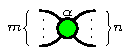
\includegraphics{generater_green_spider}
			}
			~
			\subcaptionbox{Red spider}[.2\textwidth]{%
				
\includegraphics{generater_red_spider}
			}
			~
			\subcaptionbox{Hadamard}[.2\textwidth]{%
				
\includegraphics[]{generater_hadamard}
			}
			~
			\subcaptionbox{Diamond}[.15\textwidth]{%
				
\includegraphics{generater_diamond}
			}
			%%%%%%%%%%%%%%%%%%%%%%%%%%%%%%%%%%%%%%%%
		\end{minipage}
	}
	\caption{Generators for the PROP}
	\label{fig:ZX generators}
\end{figure}
\begin{itemize}
	\item a wire with a single input and output,
	\item green nodes with a non-negative integer number of inputs and outputs and paired with a phase $\alpha \in [-\pi,\pi)$,
	\item red nodes with a non-negative integer number inputs and outputs and paired with a phase $\beta \in [-\pi,\pi)$,
	\item a yellow node with a single input and output, and
	\item a black box node with no inputs or outputs
\end{itemize}
\begin{figure}[h]
	\fbox{
		\begin{minipage}{\textwidth}
			\centering
			%%%%%%%%%%%%%%%%%%%%%%%%%%%%%%%%%%%%%%%%
			\begin{subfigure}[t]{0.4\textwidth}
				\centering
				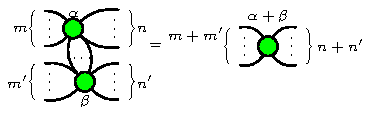
\includegraphics{equation_spider}
				\caption{Spider equation}
			\end{subfigure}%
			~
			\begin{subfigure}[t]{0.5\textwidth}
				\centering
				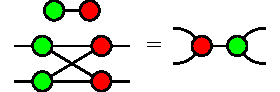
\includegraphics{equation_bialgebra}
				\caption{Bialgebra equation}
			\end{subfigure}%
			%%%%%%%%%%%%%%%%%%%%%%%%%%%%%%%%%%%%%%%%
			\vspace{2ex}
			%%%%%%%%%%%%%%%%%%%%%%%%%%%%%%%%%%%%%%%%
			\begin{subfigure}[t]{0.3\textwidth}
				\centering
				
\includegraphics{equation_loop}
				\caption{Loop equation}
			\end{subfigure}%
			~
			\begin{subfigure}[t]{0.3\textwidth}
				\centering
				
\includegraphics{equation_cup}
				\caption{Cup equation}
			\end{subfigure}%
			~
			\begin{subfigure}[t]{0.3\textwidth}
				\centering
				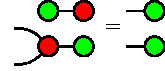
\includegraphics{equation_copy}
				\caption{Copy equation}
			\end{subfigure}%
			%%%%%%%%%%%%%%%%%%%%%%%%%%%%%%%%%%%%%%%%
			\vspace{2ex}
			%%%%%%%%%%%%%%%%%%%%%%%%%%%%%%%%%%%%%%%%
			\begin{subfigure}[t]{0.5\textwidth}
				\centering
				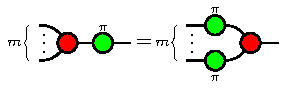
\includegraphics{equation_pi_copy}
				\caption{$\pi$-Copy equation}
			\end{subfigure}%
			~
			\begin{subfigure}[t]{0.5\textwidth}
				\centering
				
\includegraphics{equation_pi_commutation}
				\caption{$\pi$-Commutation equation}
			\end{subfigure}%
			%%%%%%%%%%%%%%%%%%%%%%%%%%%%%%%%%%%%%%%%
			\vspace{2ex}
			%%%%%%%%%%%%%%%%%%%%%%%%%%%%%%%%%%%%%%%%
			\begin{subfigure}[t]{0.5\textwidth}
				\centering
				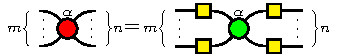
\includegraphics{equation_color_change}
				\caption{Color change equation}
			\end{subfigure}%
			~
			\begin{subfigure}[t]{0.5\textwidth}
				\centering
				\includegraphics{equation_Euler_decomposition}
				\caption{Euler decomposition equation}
			\end{subfigure}%
			%%%%%%%%%%%%%%%%%%%%%%%%%%%%%%%%%%%%%%%%
			\vspace{2ex}
			%%%%%%%%%%%%%%%%%%%%%%%%%%%%%%%%%%%%%%%%
			\begin{subfigure}[t]{0.3\textwidth}
				\centering
				\includegraphics{equation_star}
				\caption{Star equation}
			\end{subfigure}%
			~
			\begin{subfigure}[t]{0.3\textwidth}
				\centering
				\includegraphics{equation_zero}
				\caption{Zero equation}
			\end{subfigure}%
			~
			\begin{subfigure}[t]{0.3\textwidth}
				\centering
				\includegraphics{equation_zero_scalar}
				\caption{Zero scalar equation}
			\end{subfigure}%
			%%%%%%%%%%%%%%%%%%%%%%%%%%%%%%%%%%%%%%%%
		\end{minipage}
	}
	\caption{Relations in the PROP $\cat{ZX}$}
	\label{fig:ZX equations}
\end{figure}
In the spirit of compositionality, we wish to view these elements as morphisms in some category. Indeed we will now construct a dagger compact category $\cat{ZX}$ generated, in part, by the basic elements.  \todo{give credit for this category}

The objects of $\cat{ZX}$ will be the non-negative integers.  The morphisms will be generated by those depicted in Figure \ref{fig:ZX generators}, though we also include  
\[
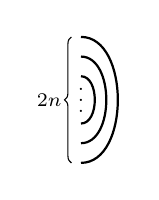
\begin{tikzpicture}[baseline=(current bounding box.base)]
	\node (1) at (0,-.85) {};
	\node (2) at (0,-0.6) {};
	\node (3) at (0,-0.35) {};
	\node (4) at (0,0.05) {\scriptsize $\vdots$};
	\node (5) at (0,0.25) {};
	\node (6) at (0,0.5) {};
	\node (7) at (0,0.75) {};
	%
	\path[-,thick]
		(1.center) edge[out=0,in=0] (7.center)
		(2.center) edge[out=0,in=0] (6.center)
		(3.center) edge[out=0,in=0] (5.center);
	%
	\draw[decoration={brace,raise=7pt},decorate]
		(1.east) -- node[left=7pt] {\scriptsize $2n$} (7.east); 
\end{tikzpicture}
\quad \text{and} \quad 
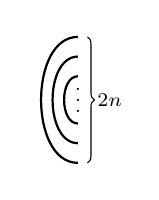
\begin{tikzpicture}[baseline=(current bounding box.base)]
	\node (1) at (0,-.85) {};
	\node (2) at (0,-0.6) {};
	\node (3) at (0,-0.35) {};
	\node (4) at (0,0.05) {\scriptsize $\vdots$};
	\node (5) at (0,0.25) {};
	\node (6) at (0,0.5) {};
	\node (7) at (0,0.75) {};
	%
	\path[-,thick]
		(1.center) edge[out=180,in=180] (7.center)
		(2.center) edge[out=180,in=180] (6.center)
		(3.center) edge[out=180,in=180] (5.center);
	\draw[decoration={brace,mirror,raise=7pt},decorate]
		(1.west) -- node[right=7pt] {\scriptsize $2n$} (7.west); 
\end{tikzpicture}
\]
to give the compact structure on the object $n$.  Their is a monoidal product on $\cat{ZX}$ given by addition on objects and disjoint union of diagrams on the morphisms.  We include another generator
\[

\begin{tikzpicture}
	\draw[thick]  plot[smooth, tension=.7] coordinates {(0.1,-0.7) (0.3,-0.6) (0.6,-0.2) (0.8,-0.1)};
	\draw[thick]  plot[smooth, tension=.7] coordinates {(0.1,-0.1) (0.3,-0.2) (0.6,-0.6) (0.8,-0.7)};
\end{tikzpicture}
\]
to provide symmetry for the monoidal product. The dagger structure is obtained by swapping inputs and outputs then, for the red and green spider diagrams, multiplying the phase by $-1$.  For instance, 
\[
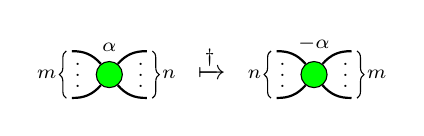
\begin{tikzpicture}
\begin{scope}[shift={(-1.3,0)}]
	\node [zxgreen,label={[shift={(0,0)}]\scriptsize $\alpha$}] (v1) at (0,0) {};
	\node (v2) at (-0.6,0.3) {};
	\node (v3) at (-0.6,-0.3) {};
	\node (v4) at (0.6,0.3) {};
	\node (v5) at (0.6,-0.3) {};
	\node at (-0.4,0.1) {\scriptsize $\vdots$};
	\node at (0.4,0.1) {\scriptsize $\vdots$};
	%
	\draw  (v1) edge [thick,bend right=25] (v2);
	\draw  (v1) edge [thick,bend left=25] (v3);
	\draw  (v1) edge [thick,bend left=25] (v4);
	\draw  (v1) edge [thick,bend right=25] (v5);
	\draw[decoration={brace,mirror,raise=2pt},decorate]
	(v2.east) -- node[left=2pt] {\scriptsize $m$} (v3.east); 
	\draw[decoration={brace,raise=2pt},decorate]
	(v4.west) -- node[right=2pt] {\scriptsize $n$} (v5.west); 
\end{scope}
%
%
%
\node at (0,0.15) {$\xmapsto{\dagger}$};
%
%
%
\begin{scope}[shift={(1.3,0)}]
	\node [zxgreen,label={[shift={(0,0)}]\scriptsize $-\alpha$}] (v1) at (0,0) {};
	\node (v2) at (-0.6,0.3) {};
	\node (v3) at (-0.6,-0.3) {};
	\node (v4) at (0.6,0.3) {};
	\node (v5) at (0.6,-0.3) {};
	\node at (-0.4,0.1) {\scriptsize $\vdots$};
	\node at (0.4,0.1) {\scriptsize $\vdots$};
	%
	\draw  (v1) edge [thick,bend right=25] (v2);
	\draw  (v1) edge [thick,bend left=25] (v3);
	\draw  (v1) edge [thick,bend left=25] (v4);
	\draw  (v1) edge [thick,bend right=25] (v5);
	\draw[decoration={brace,mirror,raise=2pt},decorate]
	(v2.east) -- node[left=2pt] {\scriptsize $n$} (v3.east); 
	\draw[decoration={brace,raise=2pt},decorate]
	(v4.west) -- node[right=2pt] {\scriptsize $m$} (v5.west); 
\end{scope}
\end{tikzpicture}
\]
The dagger acts trivially on the wire, Hadamard, and diamond elements.  

Thus far, we have a presentation for a free dagger compact category, though to obtain $\cat{ZX}$, we also include the relations depicted in Figure \ref{fig:ZX equations}. Note that, to this list of relations, we also include equations obtained  
\begin{itemize}
	\item by exchanging red and green nodes, 
	\item by daggering, and
	\item up to ambient isotopy in $4$-space.
\end{itemize}
Also, note that we denote the empty graph, which is the monoidal unit, by $\emptyset$ plus red and green nodes which are not labeled with a phase are to be considered as having a phase of $0$.  

Because th zx-calculus we cooked up to model quantum observables, there is an interpretation functor
\[
	\llbracket - \rrbracket \from \cat{ZX} \to \cat{FinHilb}_{\CC}
\]  
where $\cat{FinHilb}_{\CC}$ is the category of finite dimensional complex Hilbert spaces and linear maps. \todo{cite this} However, we are not interested in this functor.  Instead, we shall use categorify $\cat{ZX}$ using open structured graphs.

Let $S_{\text{zx}}$ be the graph 
\begin{equation}
\label{diag:zx struture graph}
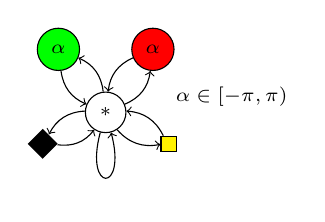
\begin{tikzpicture}[baseline=0pt]
	\node [circle,draw] (v1) at (0,0) {\scriptsize $\ast$};
	\node [zxgreen] (v2) at (-0.6,0.8) {\scriptsize $\alpha$};
	\node [zxyellow] (v3) at (0.8,-0.4) {};
	\node [zxdiamond] (v5) at (-0.8,-0.4) {};
	\node [zxred] (v4) at (0.6,0.8) {\scriptsize $\alpha$};
	\node at (1.6,0.2) {\scriptsize $\alpha \in [-\pi,\pi)$};
	%
	\draw [->]  (v1) edge [bend right] (v2);
	\draw [->] (v2) edge [bend right] (v1);
	\draw  [->](v1) edge [bend right] (v3);
	\draw [->] (v3) edge [bend right] (v1);
	\draw  [->] (v1) edge [bend right] (v4);
	\draw  [->] (v4) edge [bend right] (v1);
	\draw  [->] (v1) edge [bend right] (v5);
	\draw  [->] (v5) edge [bend right] (v1);
	\draw [<-]  (v1) edge[loop below, looseness=15] (v1);
\end{tikzpicture}
\end{equation}
We have not drawn the entirety of $S_{\text{zx}}$. Actually, for every $\alpha\in [-\pi,\pi)$, there is a green node and a red node, both which have a single arrow to and from node $\alpha$. 

Now we have the topos $\cat{Graph}/S_{\text{zx}}$ of $S_{\text{zx}}$-structured graphs. Define a functor $N_{\text{zx}} \from \cat{Set} \to \cat{Graph}/S_{\text{zx}}$ by sending a set $X$ to the edgeless $S_{\text{zx}}$-structured graph with nodes $X$ that are constant over $\ast$. We can now consider the SMCC bicategory $\cat{Rewrite}_{N,S_{\text{zx}}}$ contained in $\bimonspcsp{Graph/\text{$S_{\text{zx}}$}}$ that is full over objects of the form $N_{\text{zx}}(X)$.  Our next step is to generate a sub-bicategory inside $\cat{Rewrite}_{N_{\text{zx}},S_{\text{zx}}}$ that will categorify $\cat{ZX}$.  For this, we will first need to introduce notation.

Suppose that we have a graph morphism $f \from G \to S_{\text{zx}}$. Each node $x$ of $G$ will be drawn the in the same way as $f(x)$ is drawn in \eqref{diag:zx struture graph}. The exception is nodes in the fibre of $\ast$ which will be drawn with an open circle.  There is no need to label the arrows of $G$ because $f$ is completely determined by its behavior on the nodes. For instance, if $G$ is the graph
\[
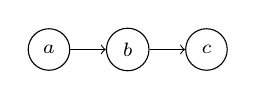
\begin{tikzpicture}
	\node [circle,draw,minimum size=1.5em] (v2) at (0,0) {\scriptsize $b$};
	\node [circle,draw,minimum size=1.5em] (v1) at (-1,0) {\scriptsize $a$};
	\node [circle,draw,minimum size=1.5em] (v3) at (1,0) {\scriptsize $c$};
	%
	\draw [->]  (v1) edge (v2);
	\draw [->] (v2) edge (v3);
\end{tikzpicture}
\] 
and $f$ is given by
\[
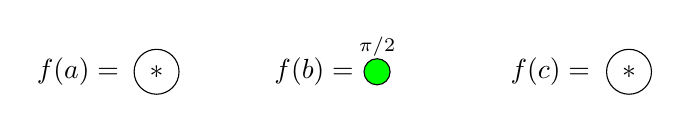
\begin{tikzpicture}
	\begin{scope}[shift={(-3,-0.6)}]
	\node at (-0.6,0) {$f(a)=$};
	\node [circle,draw] at (0.4,0) {$\ast$};
	\end{scope}
	%
	\begin{scope}
	\node at (-0.6,-0.6) {$f(b)=$};
	\node [zxgreen,label={[shift={(0,-0.1)}]\scriptsize $\pi/2$}] at (0.2,-0.6) {};
	\end{scope}
	%
	\begin{scope}[shift={(3,0.6)}]
	\node at (-0.6,-1.2) {$f(c)=$};
	\node [circle,draw] at (0.4,-1.2) {$\ast$};
	\end{scope}
\end{tikzpicture}
\]
then we draw the over object $f \from G \to S_{\text{zx}}$ as
\begin{equation}
\label{graph:over object A}
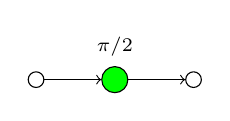
\begin{tikzpicture}
	\node [zxgreen,label={\scriptsize $\pi/2$}] (v2) at (0,0) {};
	\node [circle,draw,inner sep=2pt] (v1) at (-1,0) {};
	\node [circle,draw,inner sep=2pt] (v3) at (1,0) {};
	%
	\draw [->]  (v1) edge (v2);
	\draw [->] (v2) edge (v3);
\end{tikzpicture}
\end{equation}
However, a $1$-cell in $\cat{Rewrite}_{N_{\text{zx}},S_{\text{zx}}}$ is not just a graph over $S_{\text{zx}}$.  An object is a cospan of graphs over $S_{\text{zx}}$ such that both codomains are in the image of the node functor $N_{\text{zx}}$. To denote \eqref{graph:over object A} as an object from $N_{\text{zx}}(X) \to N_{\text{zx}}(Y)$, we write
\[
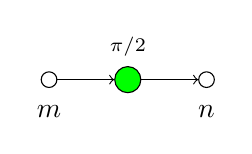
\begin{tikzpicture}
	\node [zxgreen,label={\scriptsize $\pi/2$}] (v2) at (0,0) {};
	\node [circle,draw,inner sep=2pt] (v1) at (-1,0) {};
	\node [circle,draw,inner sep=2pt] (v3) at (1,0) {};
	%
	\draw [->]  (v1) edge (v2);
	\draw [->] (v2) edge (v3);
	\node at (-1,-0.4) {$m$};
	\node at (1,-0.4) {$n$};
\end{tikzpicture}
\]
where $m = |N_{\text{zx}}(X)|$ and $n=|N_{\text{zx}}(Y)|$ as a shorthand for the cospan
\[
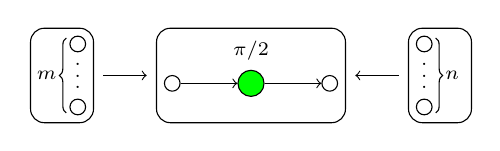
\begin{tikzpicture}
	\begin{scope}
	\node [zxgreen,label={\scriptsize $\pi/2$}] (v2) at (0,0.1) {};
	\node [circle,draw,inner sep=2pt] (v1) at (-1,0.1) {};
	\node [circle,draw,inner sep=2pt] (v3) at (1,0.1) {};
	%
	\draw [->]  (v1) edge (v2);
	\draw [->] (v2) edge (v3);
	\draw [rounded corners=5pt] (-1.2,-0.4) rectangle (1.2,0.8);
	\end{scope}
	%
	%
	%
	\begin{scope}[shift={(-2,-0.4)}]
	\node [circle,draw,inner sep=2pt] (v4) at (-0.2,0.2) {};
	\node [circle,draw,inner sep=2pt] (v5) at (-0.2,1) {};
	\node at (-0.2,0.7) {\scriptsize $\vdots$};
	\draw [rounded corners=5pt] (-0.8,0) rectangle (0,1.2);
	\draw[decoration={brace,raise=2pt},decorate]
	(v4.south west) -- node [left=2pt] {\scriptsize $m$} (v5.north west); 
	\end{scope}
	%
	%
	%
	\begin{scope}[shift={(2.8,-0.4)}]
	\node [circle,draw,inner sep=2pt] (v4) at (-0.6,0.2) {};
	\node [circle,draw,inner sep=2pt] (v5) at (-0.6,1) {};
	\node at (-0.6,0.7) {\scriptsize $\vdots$};
	\draw [rounded corners=5pt] (-0.8,0) rectangle (0,1.2);
	\draw[decoration={brace,mirror,raise=2pt},decorate]
	(v4.south east) -- node [right=2pt] {\scriptsize $n$} (v5.north east); 
	\end{scope}
	%
	\node (v6) at (-2,0.2) {};
	\node (v7) at (-1.2,0.2) {};
	\node (v8) at (2,0.2) {};
	\node (v9) at (1.2,0.2) {};
	\draw [->] (v6) edge (v7);
	\draw [->] (v8) edge (v9);
\end{tikzpicture}
\]
of graphs over $S_{\text{zx}}$.  In this example, the graph maps in the cospan are clear and, indeed, suppressing the behavior of the maps in our shorthand should not lead to confusion. 

We are now ready to give a presentation of $\underline{\cat{ZX}}$. 



 \todo{put more language here}

\begin{figure}[h]
	\fbox{%
		\begin{minipage}{\textwidth}
			\centering
			%%%%%%%%%%%%%%%%%%%%%%%%%%%%%%%%%%%%%%%%
			\subcaptionbox{Wire}[.30\textwidth]{%
				\includegraphics{1cell_wire}
			}
			~
			\subcaptionbox{Hadamard}[.30\textwidth]{%
				\includegraphics[]{1cell_hadamard}
			}
			~
			\subcaptionbox{Diamond}[.30\textwidth]{%
				\includegraphics{1cell_diamond}
			}
			\linebreak
			\subcaptionbox{Green spider}[.4\textwidth]{%
				\includegraphics{1cell_green_spider}
			}
			~
			\subcaptionbox{Red spider}[.4\textwidth]{%
				\includegraphics{1cell_red_spider}
			}
			%%%%%%%%%%%%%%%%%%%%%%%%%%%%%%%%%%%%%%%%
		\end{minipage}
	}
	\caption{Generating $1$-cells }
	\label{fig:ZX 1cells generators}
\end{figure}

\begin{figure}[h]
	\fbox{%
		\begin{minipage}{\textwidth}
			\centering
			%%%%%%%%%%%%%%%%%%%%%%%%%%%%%%%%%%%%%%%%
			\subcaptionbox{Spider}[\textwidth]{%
				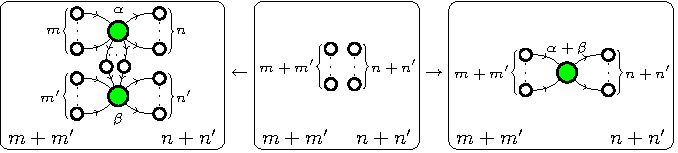
\includegraphics[scale=0.8]{2cell_spider}
			}
			\linebreak 
			\subcaptionbox{Loop}[\textwidth]{%
				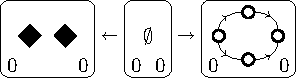
\includegraphics[scale=0.8]{2cell_loop}
			}
			\linebreak
			\subcaptionbox{Cup}[0.45\textwidth]{%
				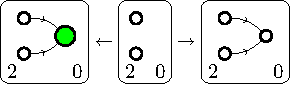
\includegraphics[scale=0.8]{2cell_cup}
			}
			\subcaptionbox{Copy}[0.45\textwidth]{%
				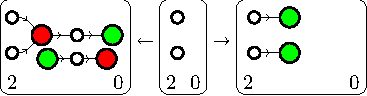
\includegraphics[scale=0.8]{2cell_copy}
			}
			\linebreak
			\subcaptionbox{Bialgebra}[\textwidth]{%
				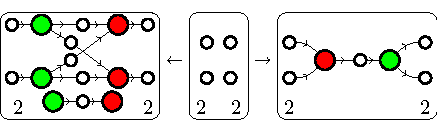
\includegraphics[scale=0.8]{2cell_bialgebra}
			}
			\linebreak
			\subcaptionbox{$\pi$-copy}[\textwidth]{%
				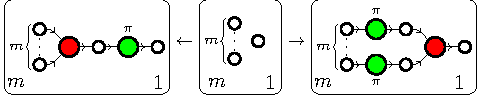
\includegraphics[scale=0.8]{2cell_pi_copy}
			}
			\linebreak
			\subcaptionbox{$\pi$-commutation}[\textwidth]{%
				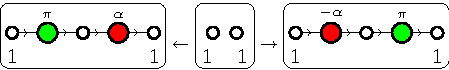
\includegraphics[scale=0.8]{2cell_pi_commutation}
			}
			\linebreak
			\subcaptionbox{Color change}[\textwidth]{%
				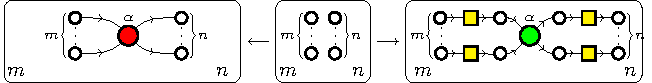
\includegraphics[scale=0.8]{2cell_color_change}
			}
			\linebreak
			\subcaptionbox{Euler decomposition}[\textwidth]{%
				\includegraphics[scale=0.8]{2cell_euler_decomposition}
			}
			\linebreak
			\subcaptionbox{diamond}[0.45\textwidth]{%
				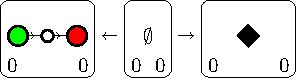
\includegraphics[scale=0.8]{2cell_diamond}
			}
			\subcaptionbox{Zero scalar}[0.45\textwidth]{%
				\includegraphics[scale=0.8]{2cell_zero_scalar}
			}
			\linebreak
			\subcaptionbox{Zero}[\textwidth]{%
				\includegraphics[scale=0.8]{2cell_zero}
			}
			\linebreak
			%%%%%%%%%%%%%%%%%%%%%%%%%%%%%%%%%%%%%%%%
		\end{minipage}
	}
	\caption{Generating $2$-cells}
	\label{fig:ZX 2cells generators}
\end{figure}

 

\begin{thm}
	The decategorification of the bicategory $\cat{zxRewrite}$ to a category is equivalent to the category $\cat{ZX}$.
\end{thm}
\begin{proof}
	\todo{prove this sucker}
\end{proof}





%%%%%%%%%%%%%%%%%%%%%%%%%%%%%%%%%%%%%%%%%%%%%%%%%%%%%%%%%%
%%%%%%%%%%%%%%%%%%%%%%%%%%%%%%%%%%%%%%%%%%%%%%%%%%%%%%%%%%
%
% BIBLIOGRAPHY
%
%%%%%%%%%%%%%%%%%%%%%%%%%%%%%%%%%%%%%%%%%%%%%%%%%%%%%%%%%%
%%%%%%%%%%%%%%%%%%%%%%%%%%%%%%%%%%%%%%%%%%%%%%%%%%%%%%%%%%

%\bibliographystyle{abbrv}
\begin{thebibliography}{100}	
	\bibitem{Cic} 
	D.~Cicala, 
	Spans of cospans.
	Available as \href{https://arxiv.org/abs/1611.07886}{arXiv:1611.07886}.
\end{thebibliography}


%%%%%%%%%%%%%%%%%%%%%%%%%%%%%%%%%%%%%%%%%%%%%%%%%%%%%%%%%
%%%%%%%%%%%%%%%%%%%%%%%%%%%%%%%%%%%%%%%%%%%%%%%%%%%%%%%%%
%%%%%%%%%%%%%%%%%%%%%%%%%%%%%%%%%%%%%%%%%%%%%%%%%%%%%%%%%
%%%%%%%%%%%%%%%%%%%%%%%%%%%%%%%%%%%%%%%%%%%%%%%%%%%%%%%%%
%
% END DOCUMENT
%
%%%%%%%%%%%%%%%%%%%%%%%%%%%%%%%%%%%%%%%%%%%%%%%%%%%%%%%%%
%%%%%%%%%%%%%%%%%%%%%%%%%%%%%%%%%%%%%%%%%%%%%%%%%%%%%%%%%
%%%%%%%%%%%%%%%%%%%%%%%%%%%%%%%%%%%%%%%%%%%%%%%%%%%%%%%%%
%%%%%%%%%%%%%%%%%%%%%%%%%%%%%%%%%%%%%%%%%%%%%%%%%%%%%%%%%

\end{document}
